\section{Introducción a Comunicacion LoRa (Comandos AT)}

\begin{figure}[H]
    \centering
    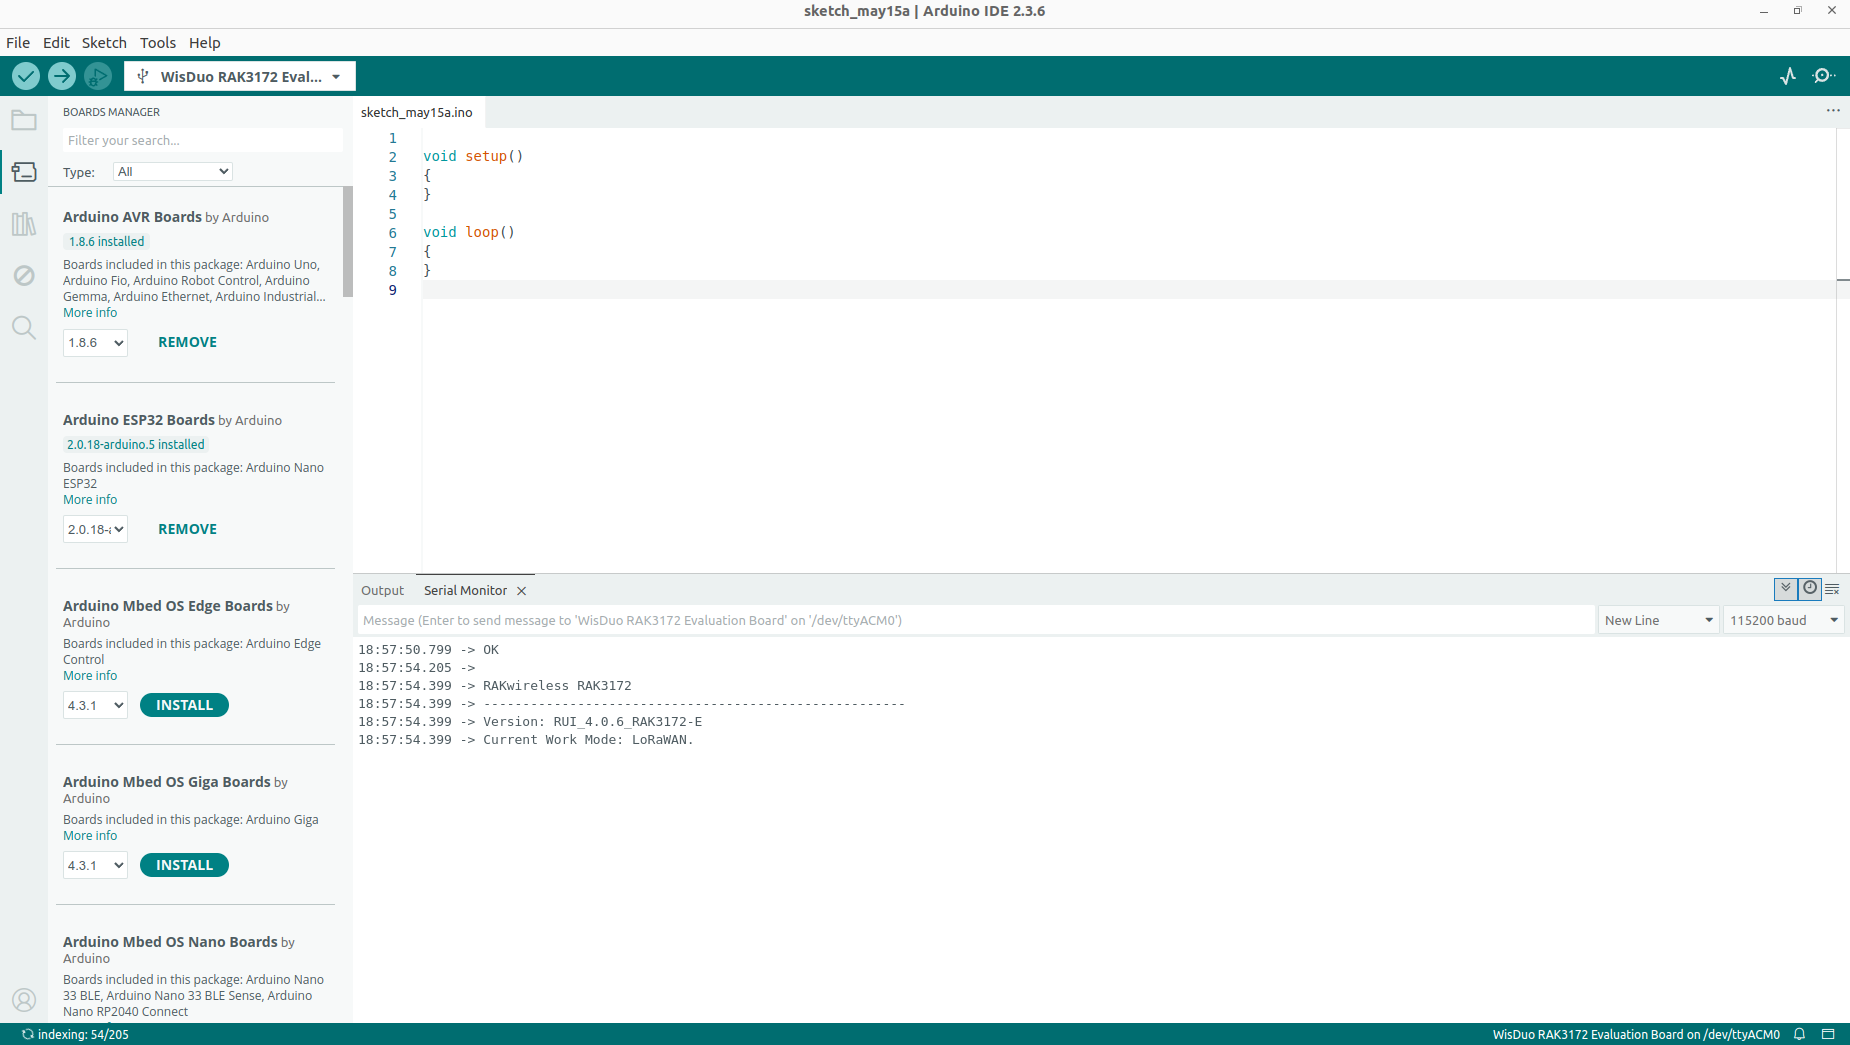
\includegraphics[width=0.85\textwidth]{./img/AT_command.png}
    \caption{...}
    \label{fig:at_command}
\end{figure}

% TODO: desarrollo de la experiencia


\section{Carga de Codigo de Prueba a RAK3172S}

\begin{figure}[H]
    \centering
    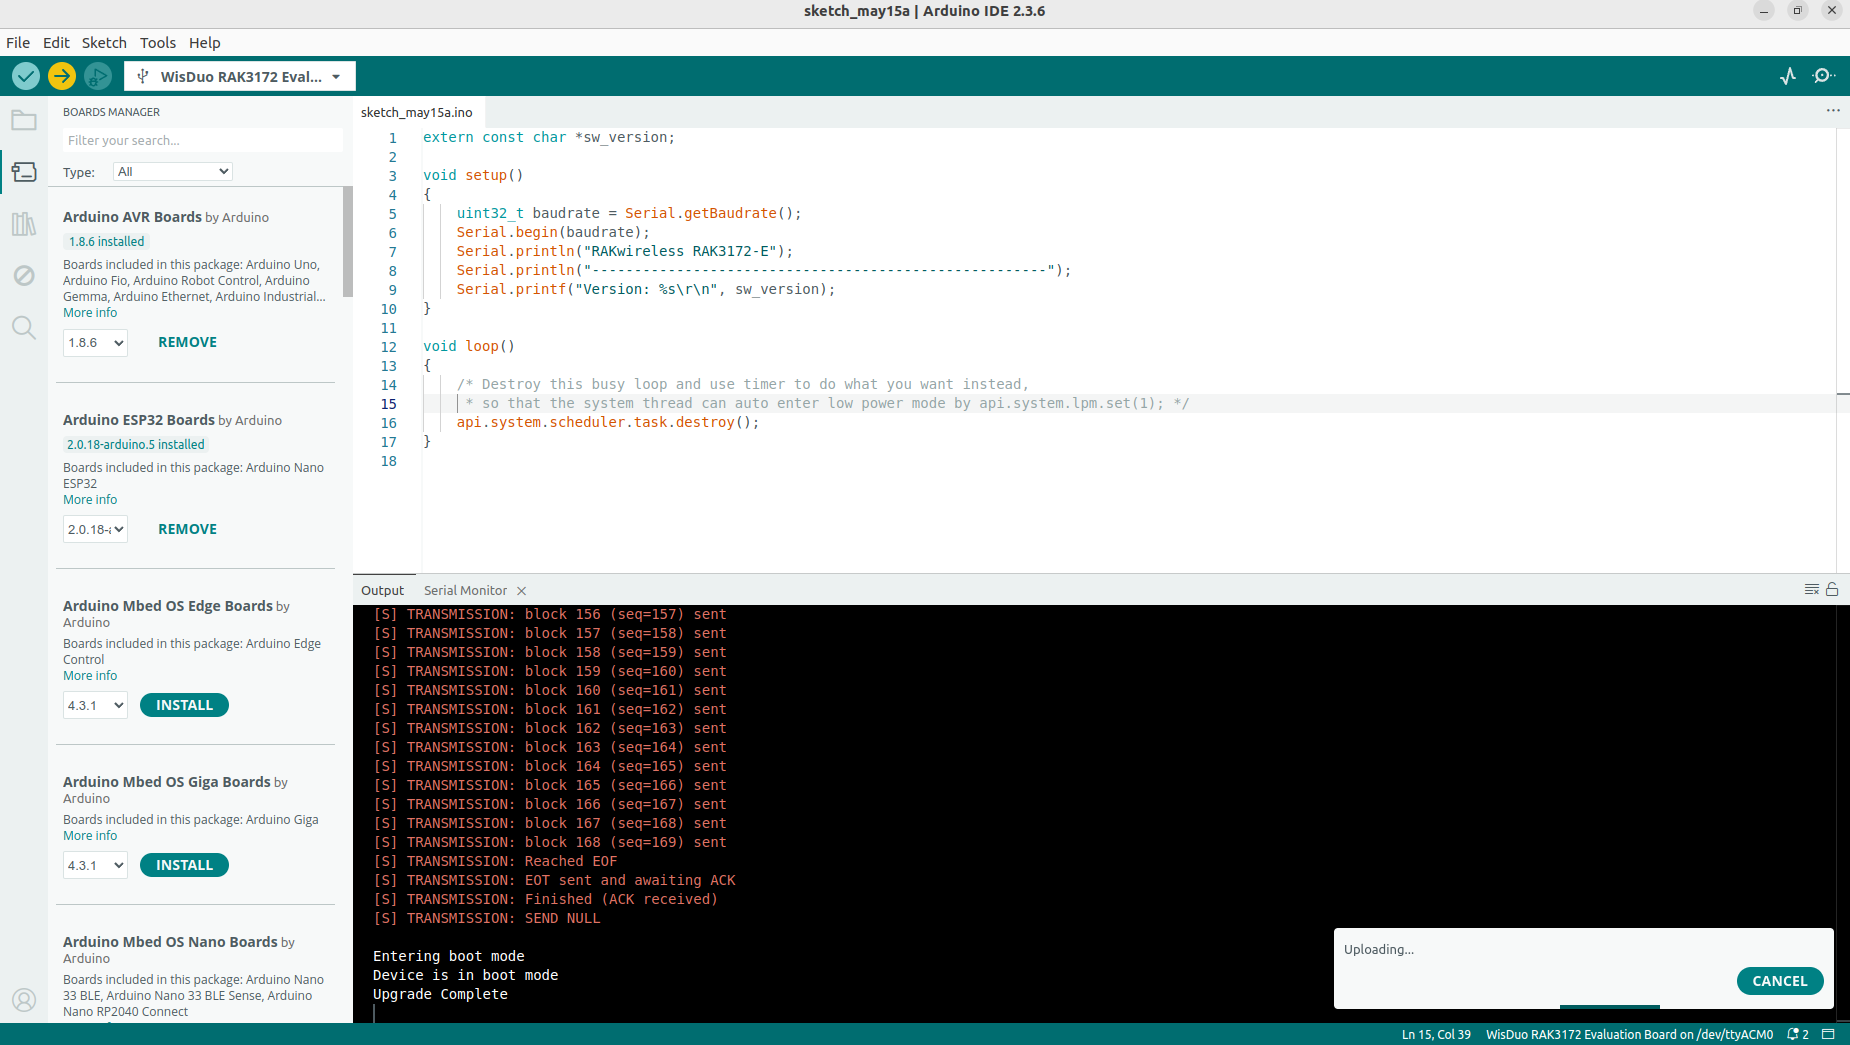
\includegraphics[width=0.85\textwidth]{./img/codigo_prueba.png}
    \caption{...}
    \label{fig:codigo_prueba}
\end{figure}

% TODO: desarrollo de la experiencia

\section{Implementacion del sistema de comunicacion P2P con LoRa}


\subsection{Transmisor}

\begin{figure}[H]
    \centering
    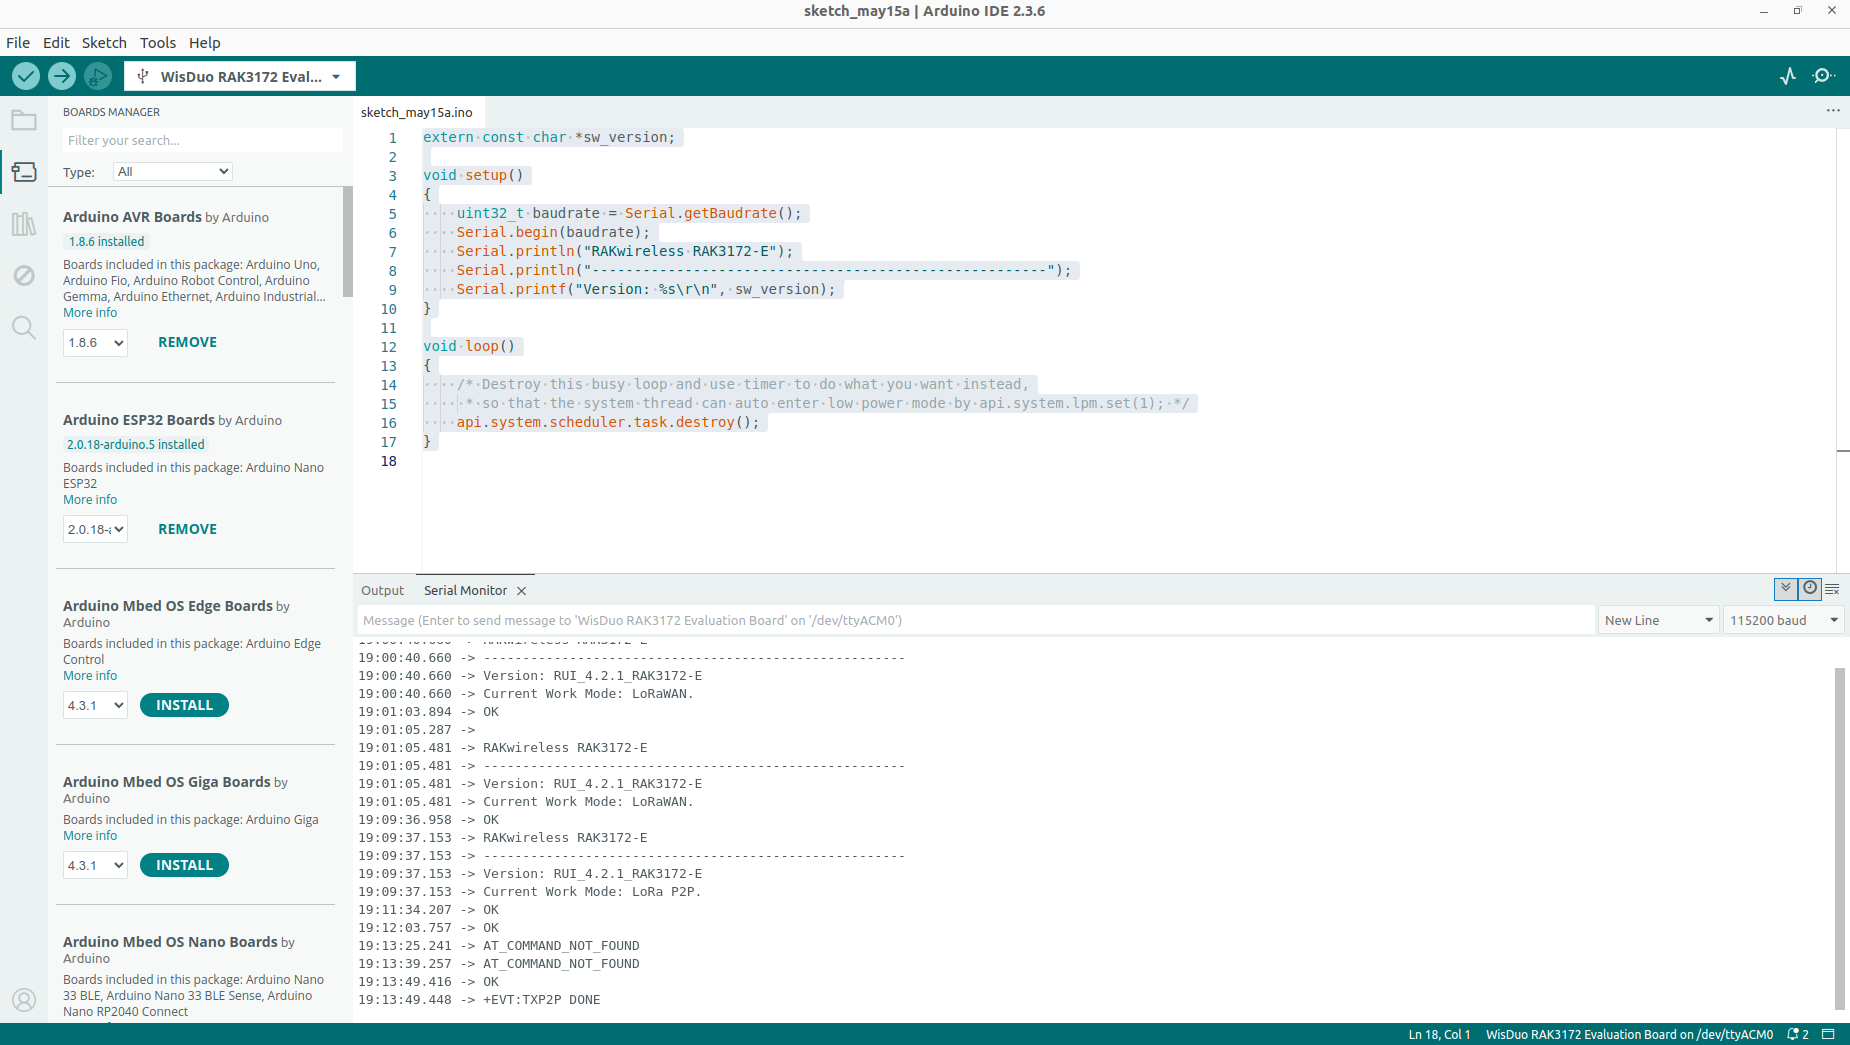
\includegraphics[width=0.85\textwidth]{./img/transmisor_setup.png}
    \caption{...}
    \label{fig:transmisor_setup}
\end{figure}

\begin{figure}[H]
    \centering
    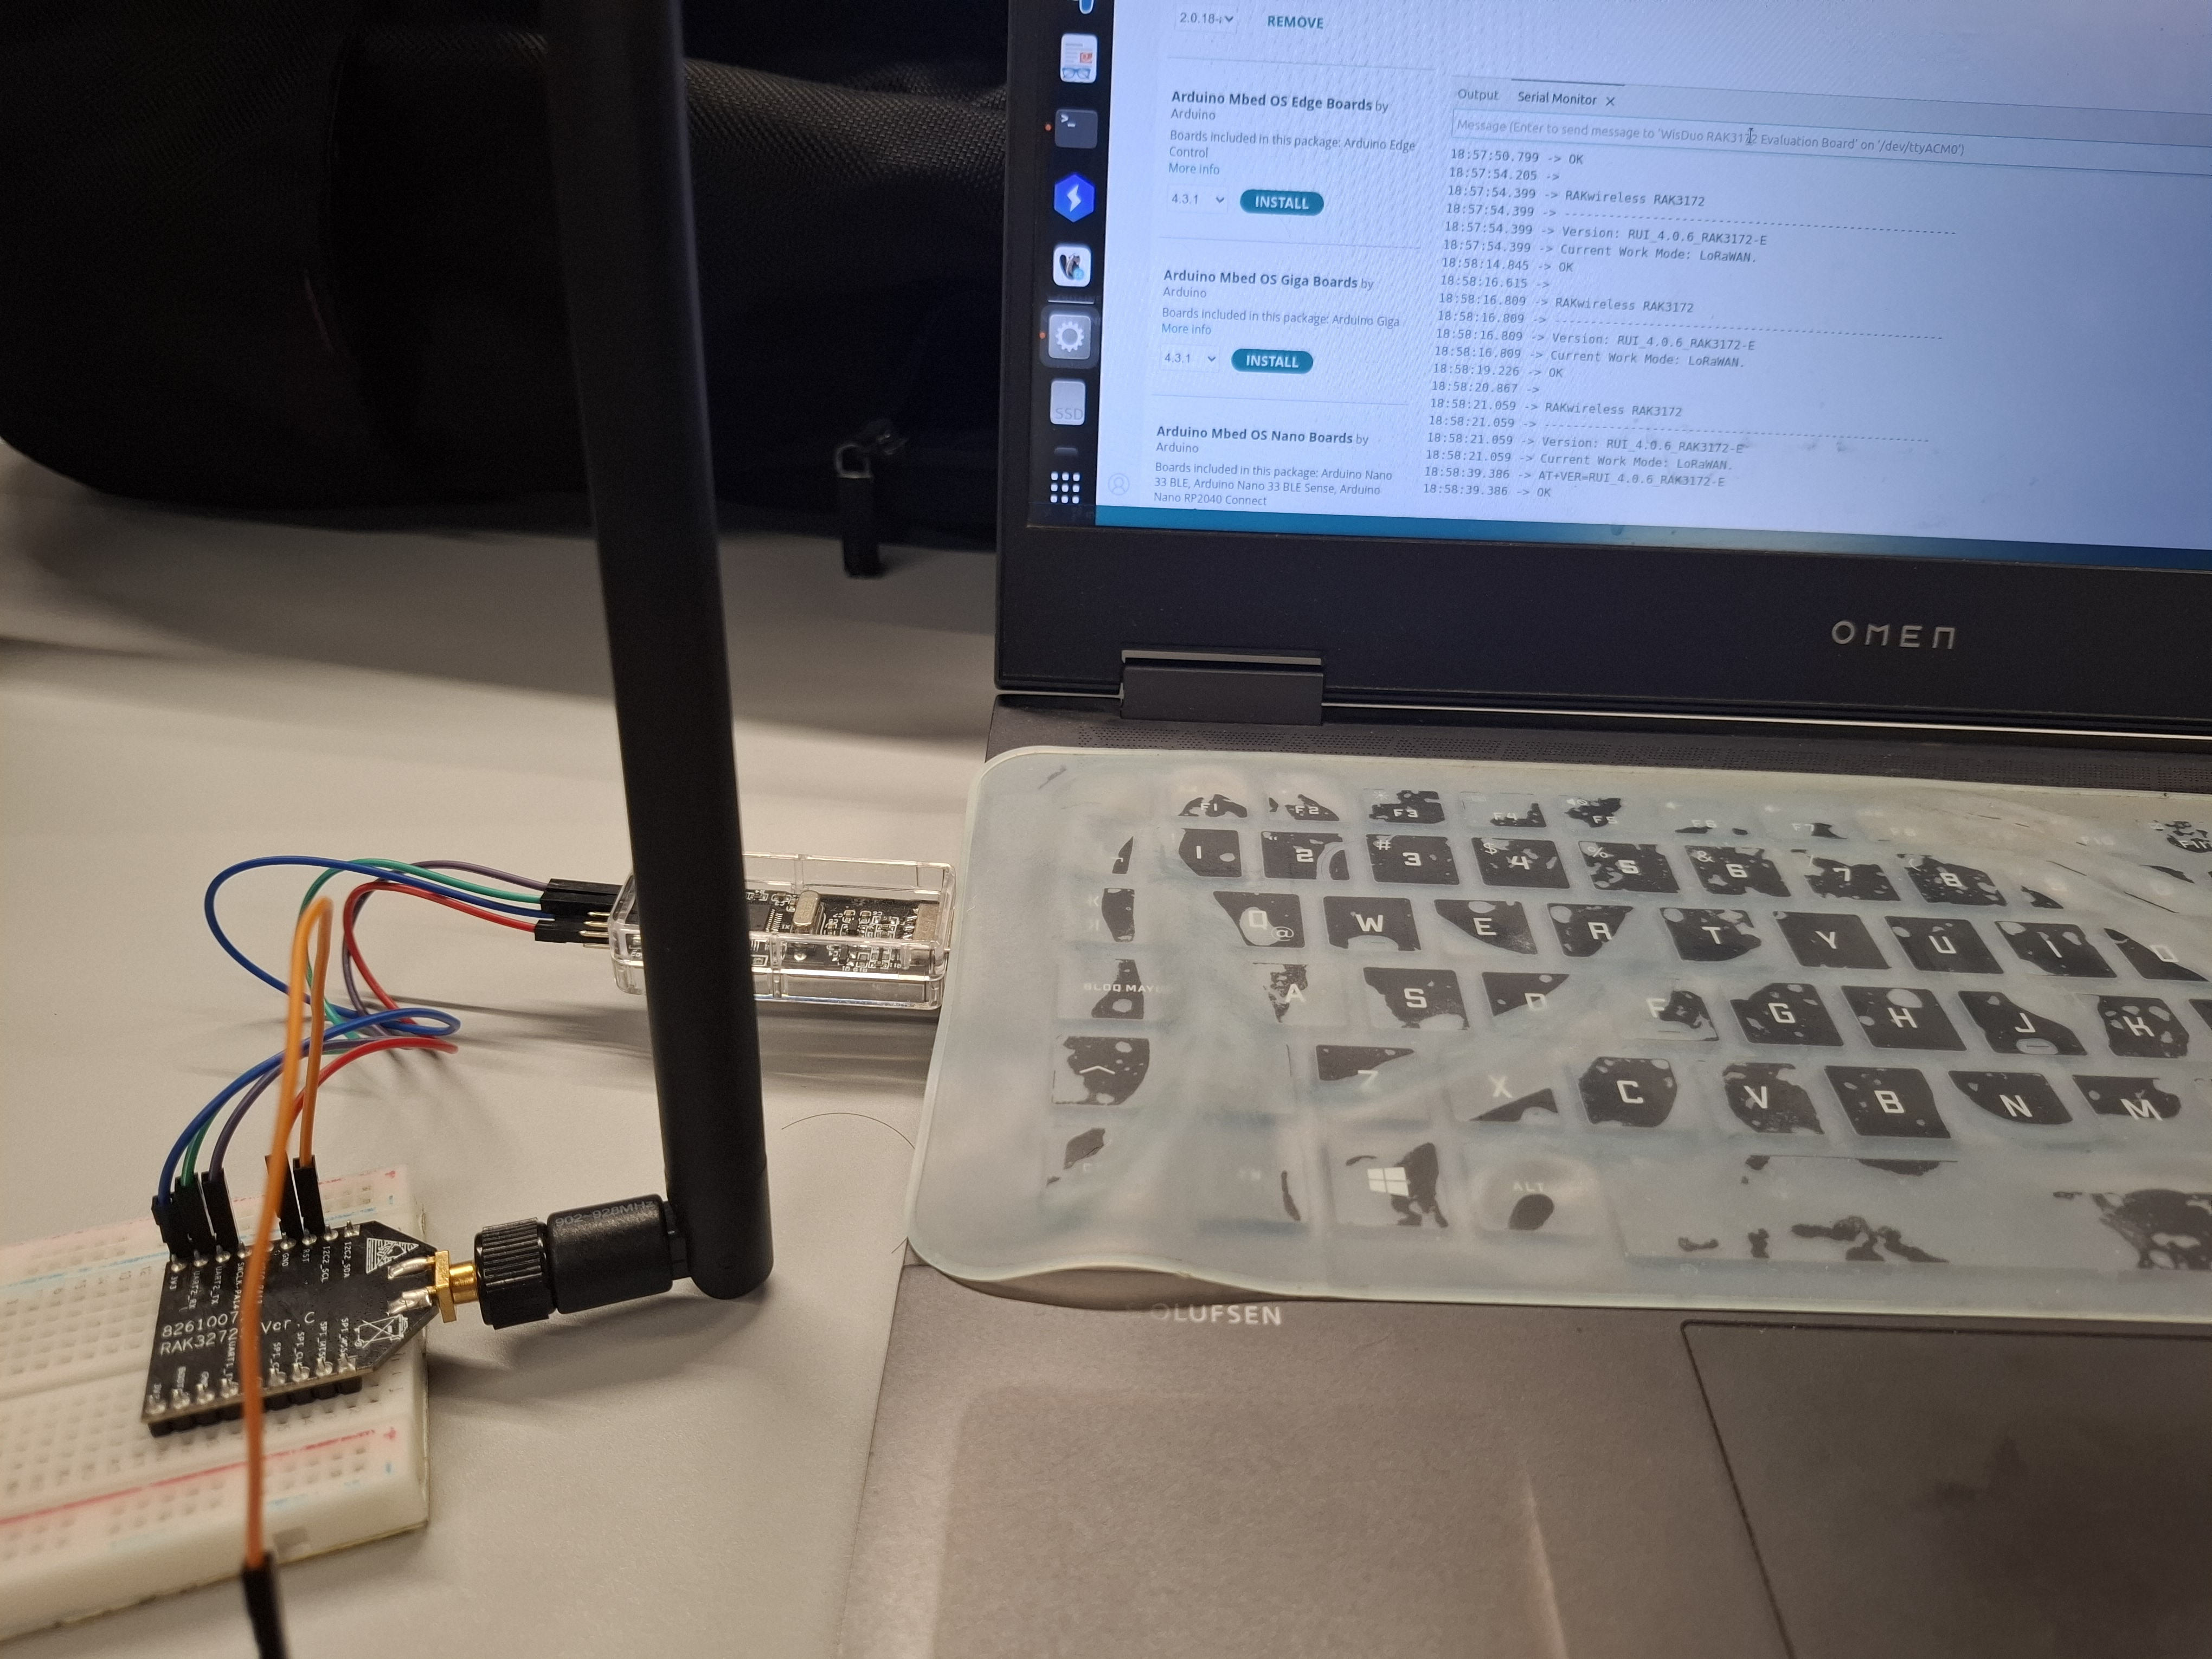
\includegraphics[width=0.85\textwidth]{./img/transmisor.jpg}
    \caption{...}
    \label{fig:transmisor_impl}
\end{figure}



\begin{figure}[H]
    \centering
    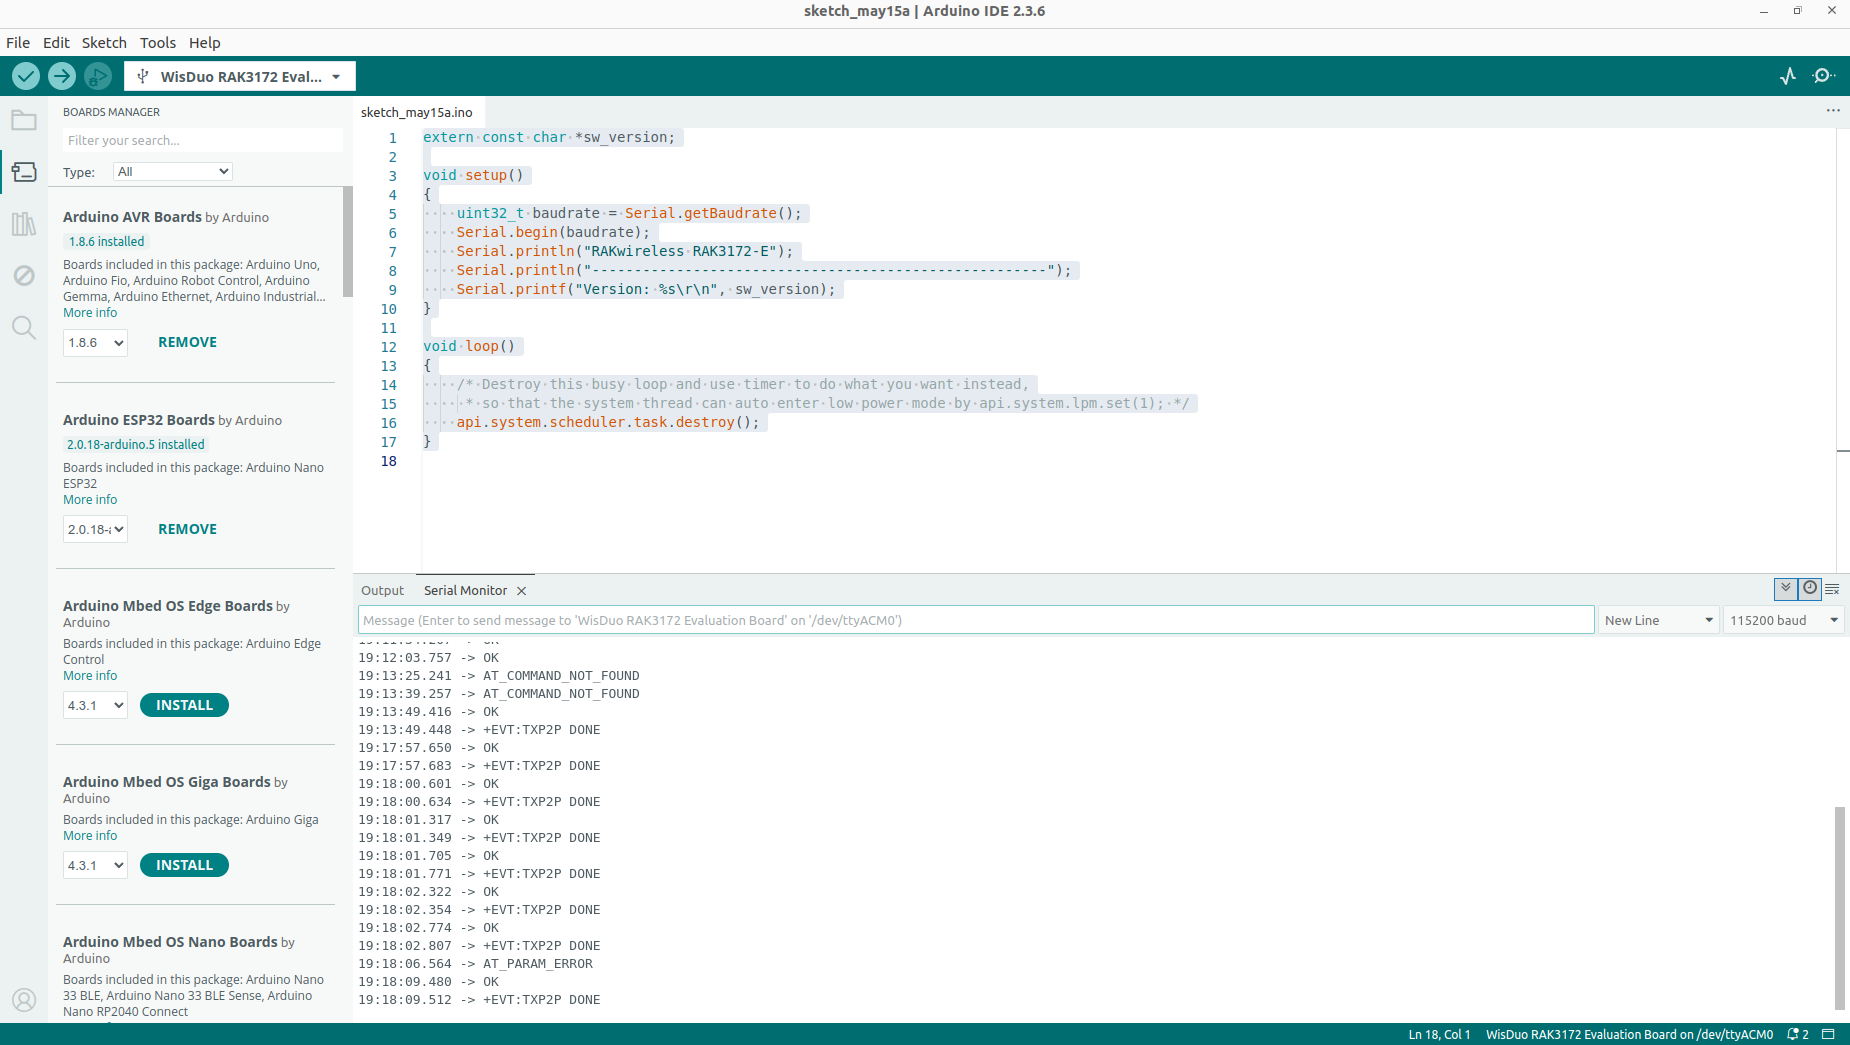
\includegraphics[width=0.85\textwidth]{./img/transmisor_envio_mnsjs.png}
    \caption{...}
    \label{fig:transmisor_envio_mnsjs}
\end{figure}


\subsection{Receptor}

% TODO: Receptor
% TODO: desarrollo de la experiencia


\section{Implementacion del sistema de comunicacion P2P con LoRa, integrado con Arduino y un sensor}


\begin{figure}[H]
    \centering
    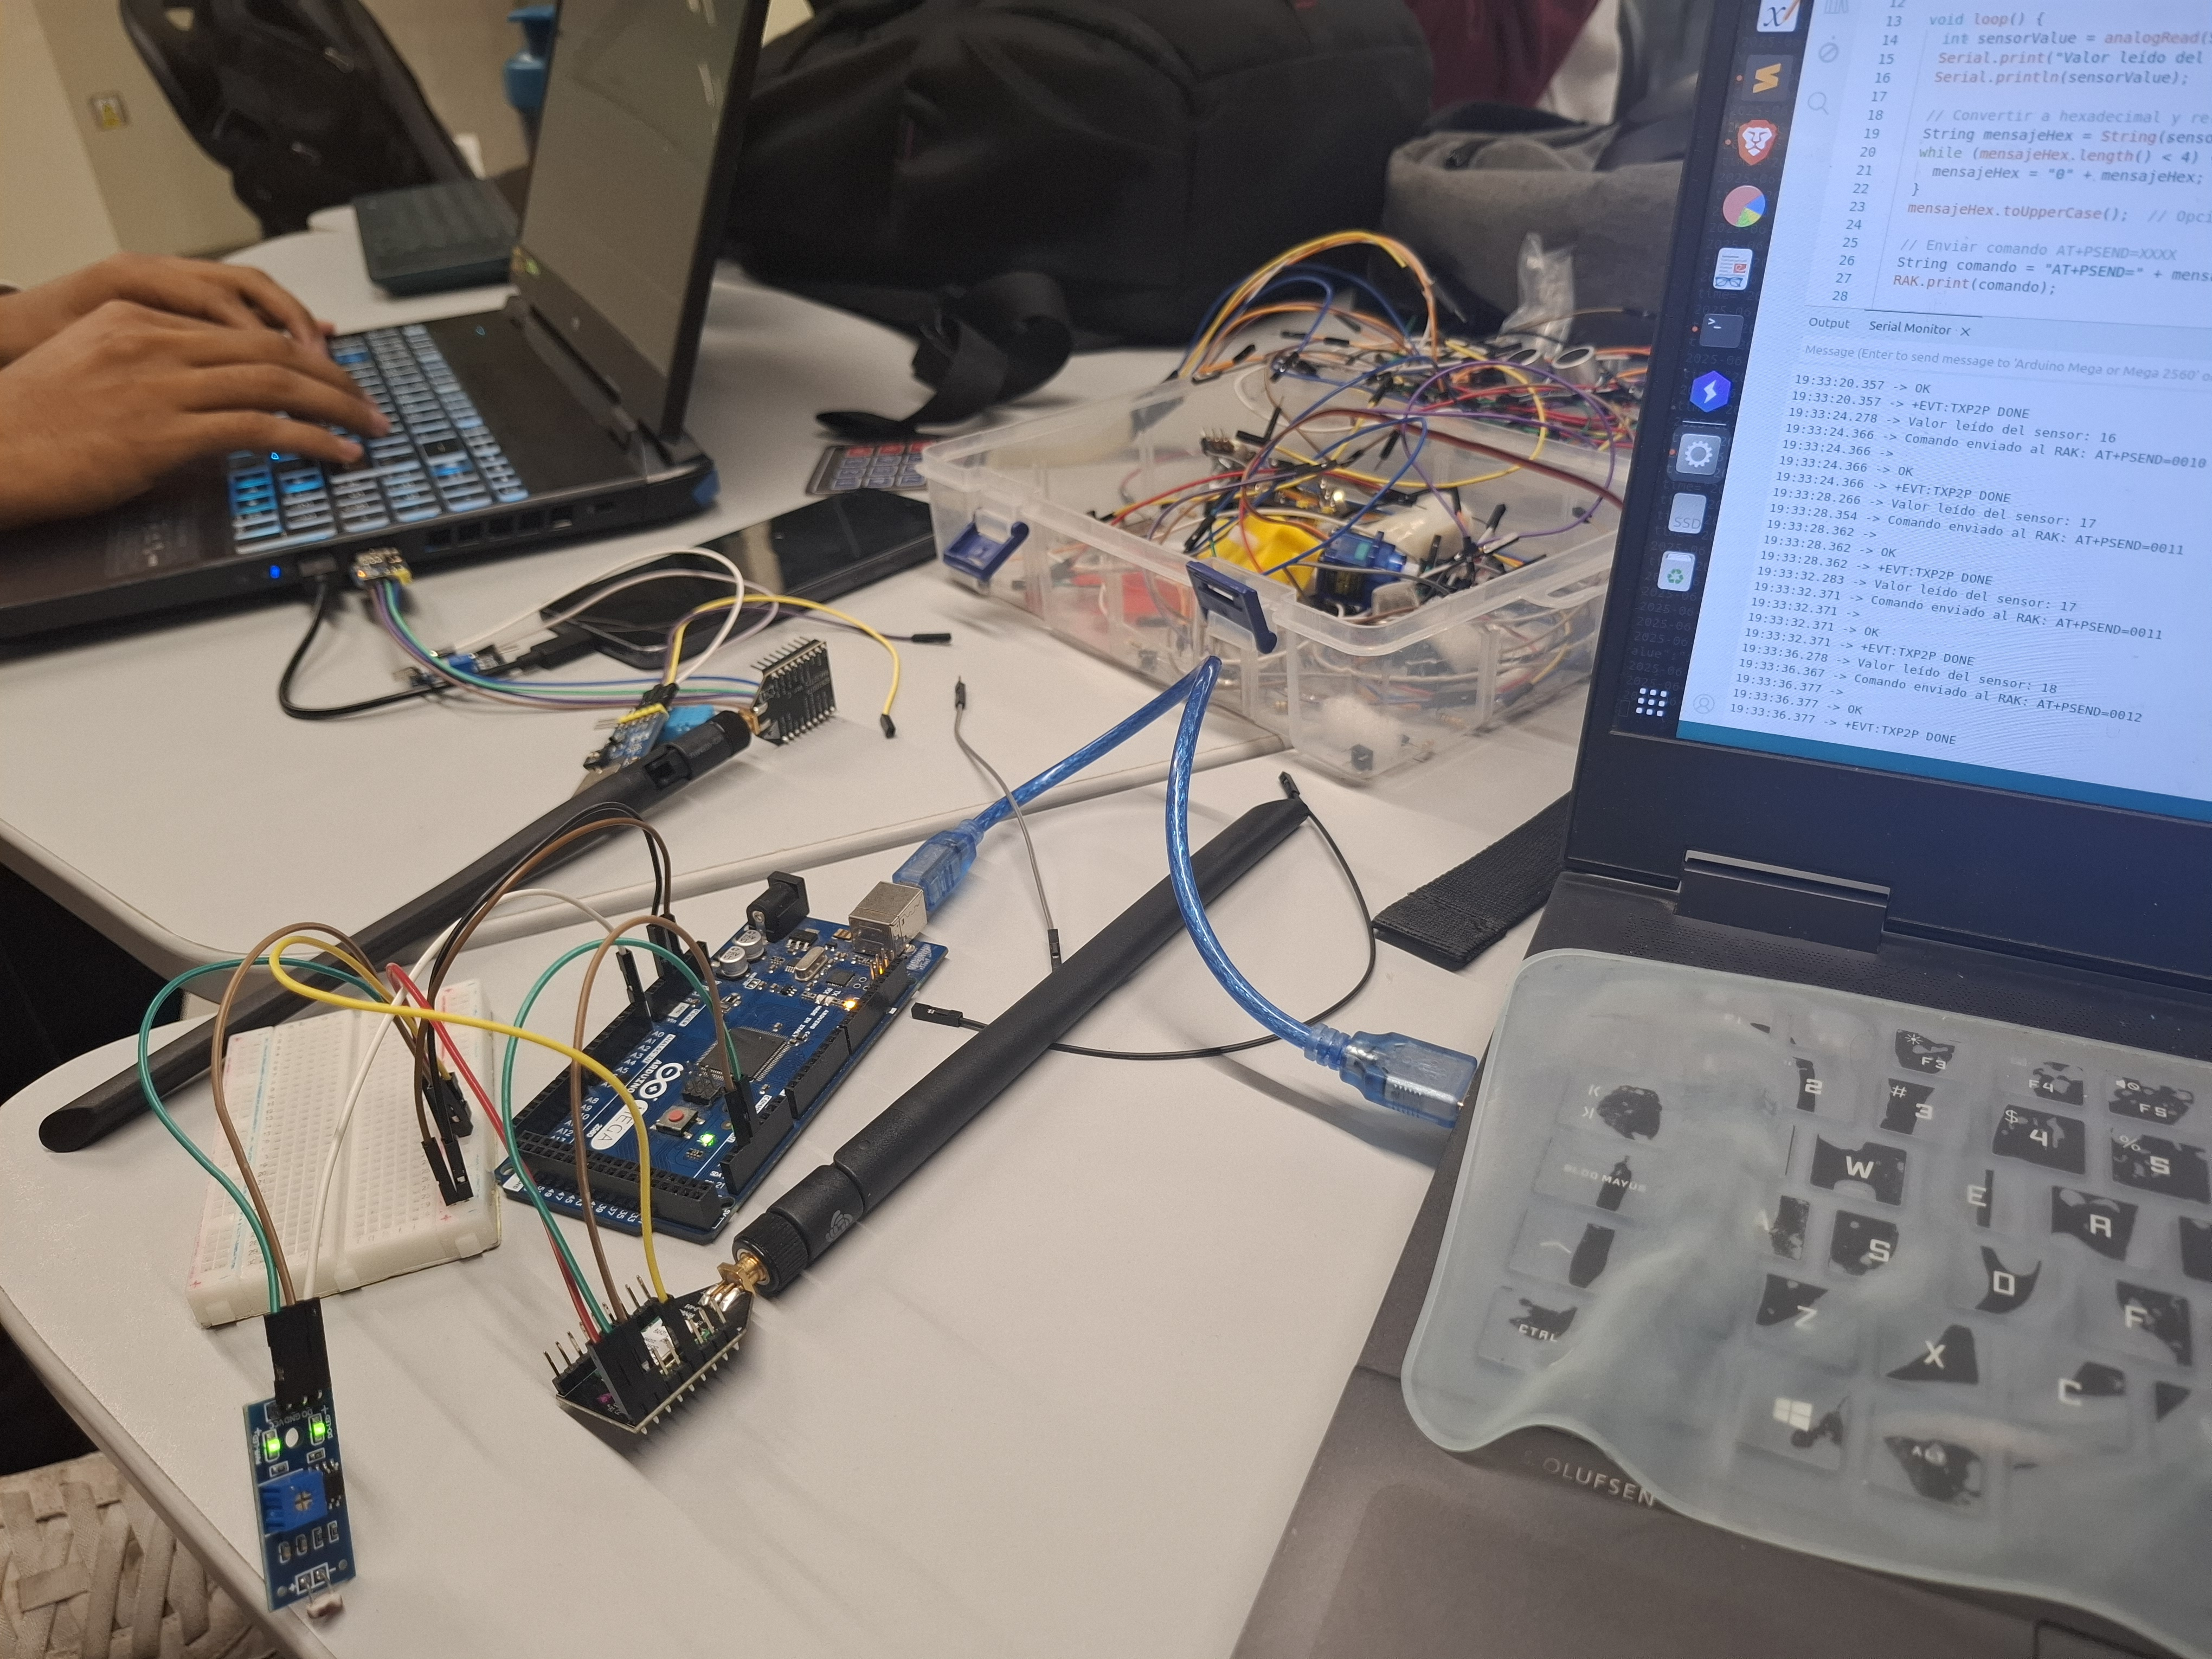
\includegraphics[width=0.85\textwidth]{./img/emisor_arduino.jpg}
    \caption{...}
    \label{fig:emisor_arduino}
\end{figure}


\begin{figure}[H]
    \centering
    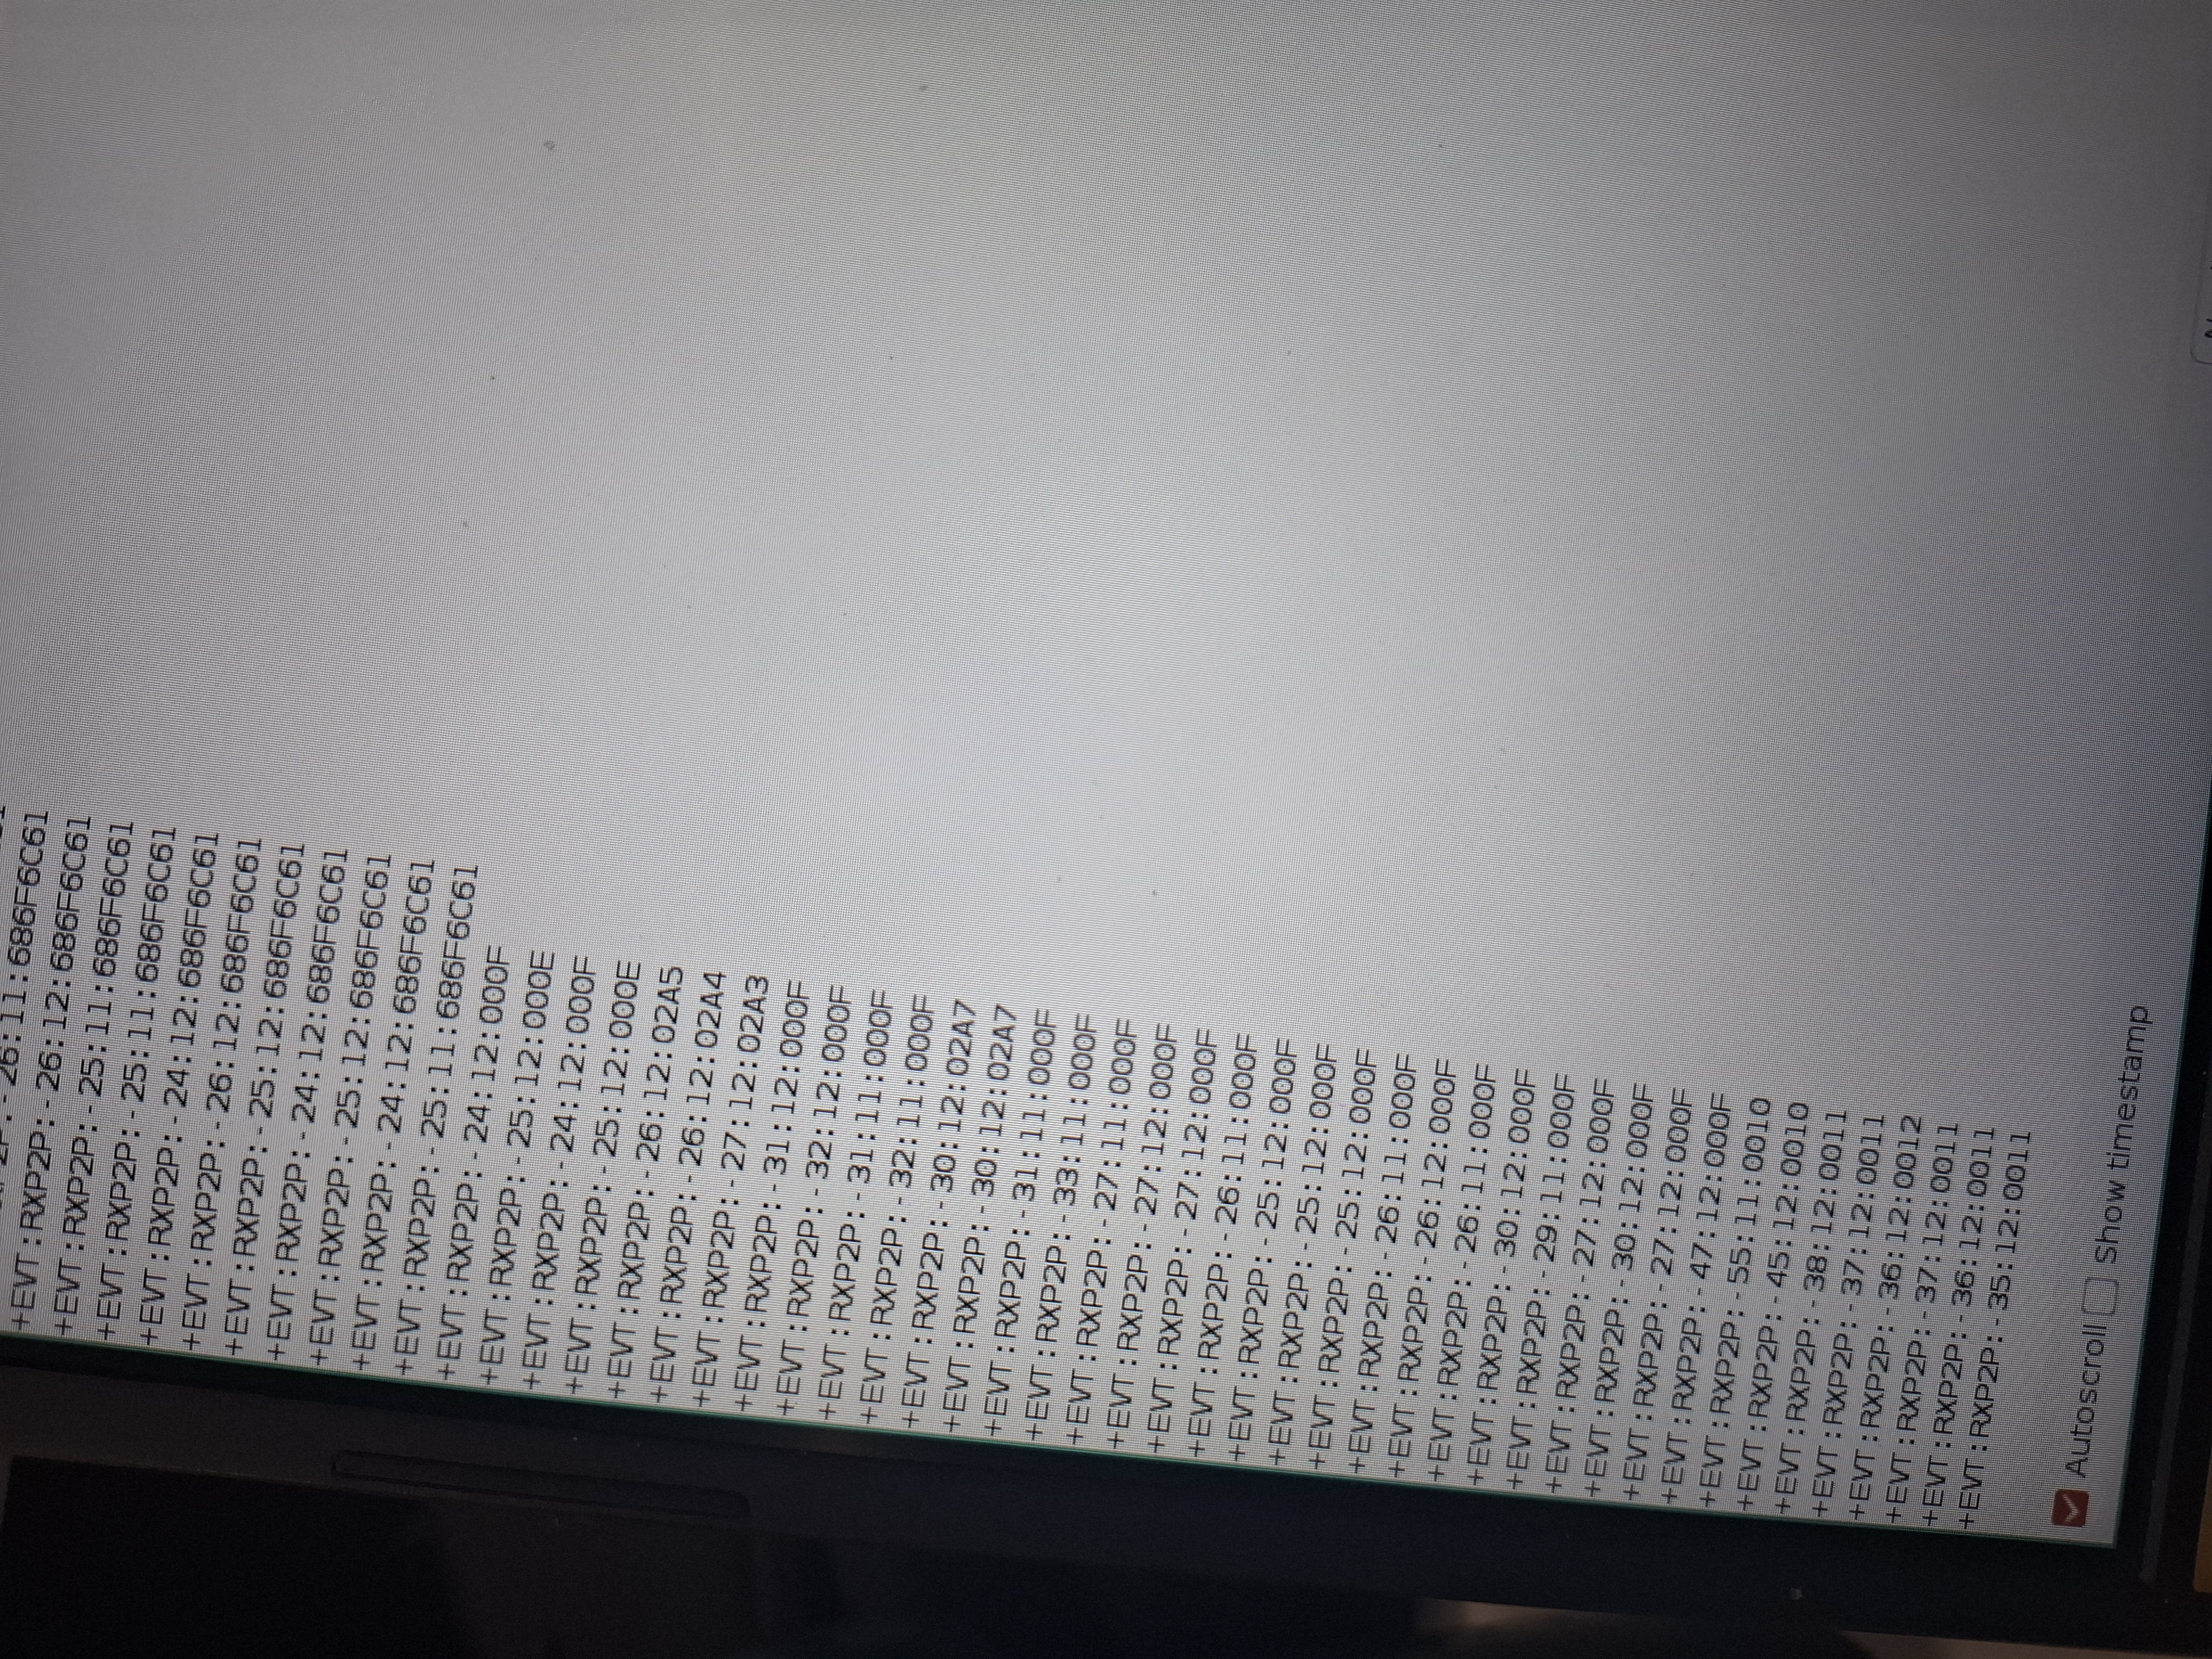
\includegraphics[width=0.85\textwidth]{./img/receptor_arduino.jpg}
    \caption{...}
    \label{fig:receptor_arduino}
\end{figure}


\begin{lstlisting}[style=cppstyle]
#define SENSOR_PIN A0       // Pin del sensor
#define RAK Serial1         // Puerto conectado al RAK (TX1/RX1)
#define BAUD_PC 9600        // Velocidad para PC
#define BAUD_RAK 115200     // Velocidad del RAK3172

void setup() {
  Serial.begin(BAUD_PC);    // Comunicación con la PC
  RAK.begin(BAUD_RAK);      // Comunicación con el RAK3172
  delay(1000);
  Serial.println("Inicio de transmisión LoRa con datos del sensor...");
}

void loop() {
  int sensorValue = analogRead(SENSOR_PIN);  // Lectura (0 a 1023)
  Serial.print("Valor leído del sensor: ");
  Serial.println(sensorValue);

  // Convertir a hexadecimal y rellenar a 4 dígitos con ceros
  String mensajeHex = String(sensorValue, HEX);
  while (mensajeHex.length() < 4) {
    mensajeHex = "0" + mensajeHex;
  }
  mensajeHex.toUpperCase();  // Opcional: para mantener todo en mayúsculas

  // Enviar comando AT+PSEND=XXXX
  String comando = "AT+PSEND=" + mensajeHex + "\r\n";
  RAK.print(comando);

  Serial.print("Comando enviado al RAK: ");
  Serial.println(comando);

  // Leer respuesta del RAK
  unsigned long start = millis();
  while (millis() - start < 1000) {
    while (RAK.available()) {
      char c = RAK.read();
      Serial.write(c);
    }
  }

  delay(3000);  // Esperar antes de enviar de nuevo
}
\end{lstlisting}

% TODO: codigo y fotos

\section{Sistema IoT de alerta de fuga de gas}

\begin{figure}[H]
    \centering
    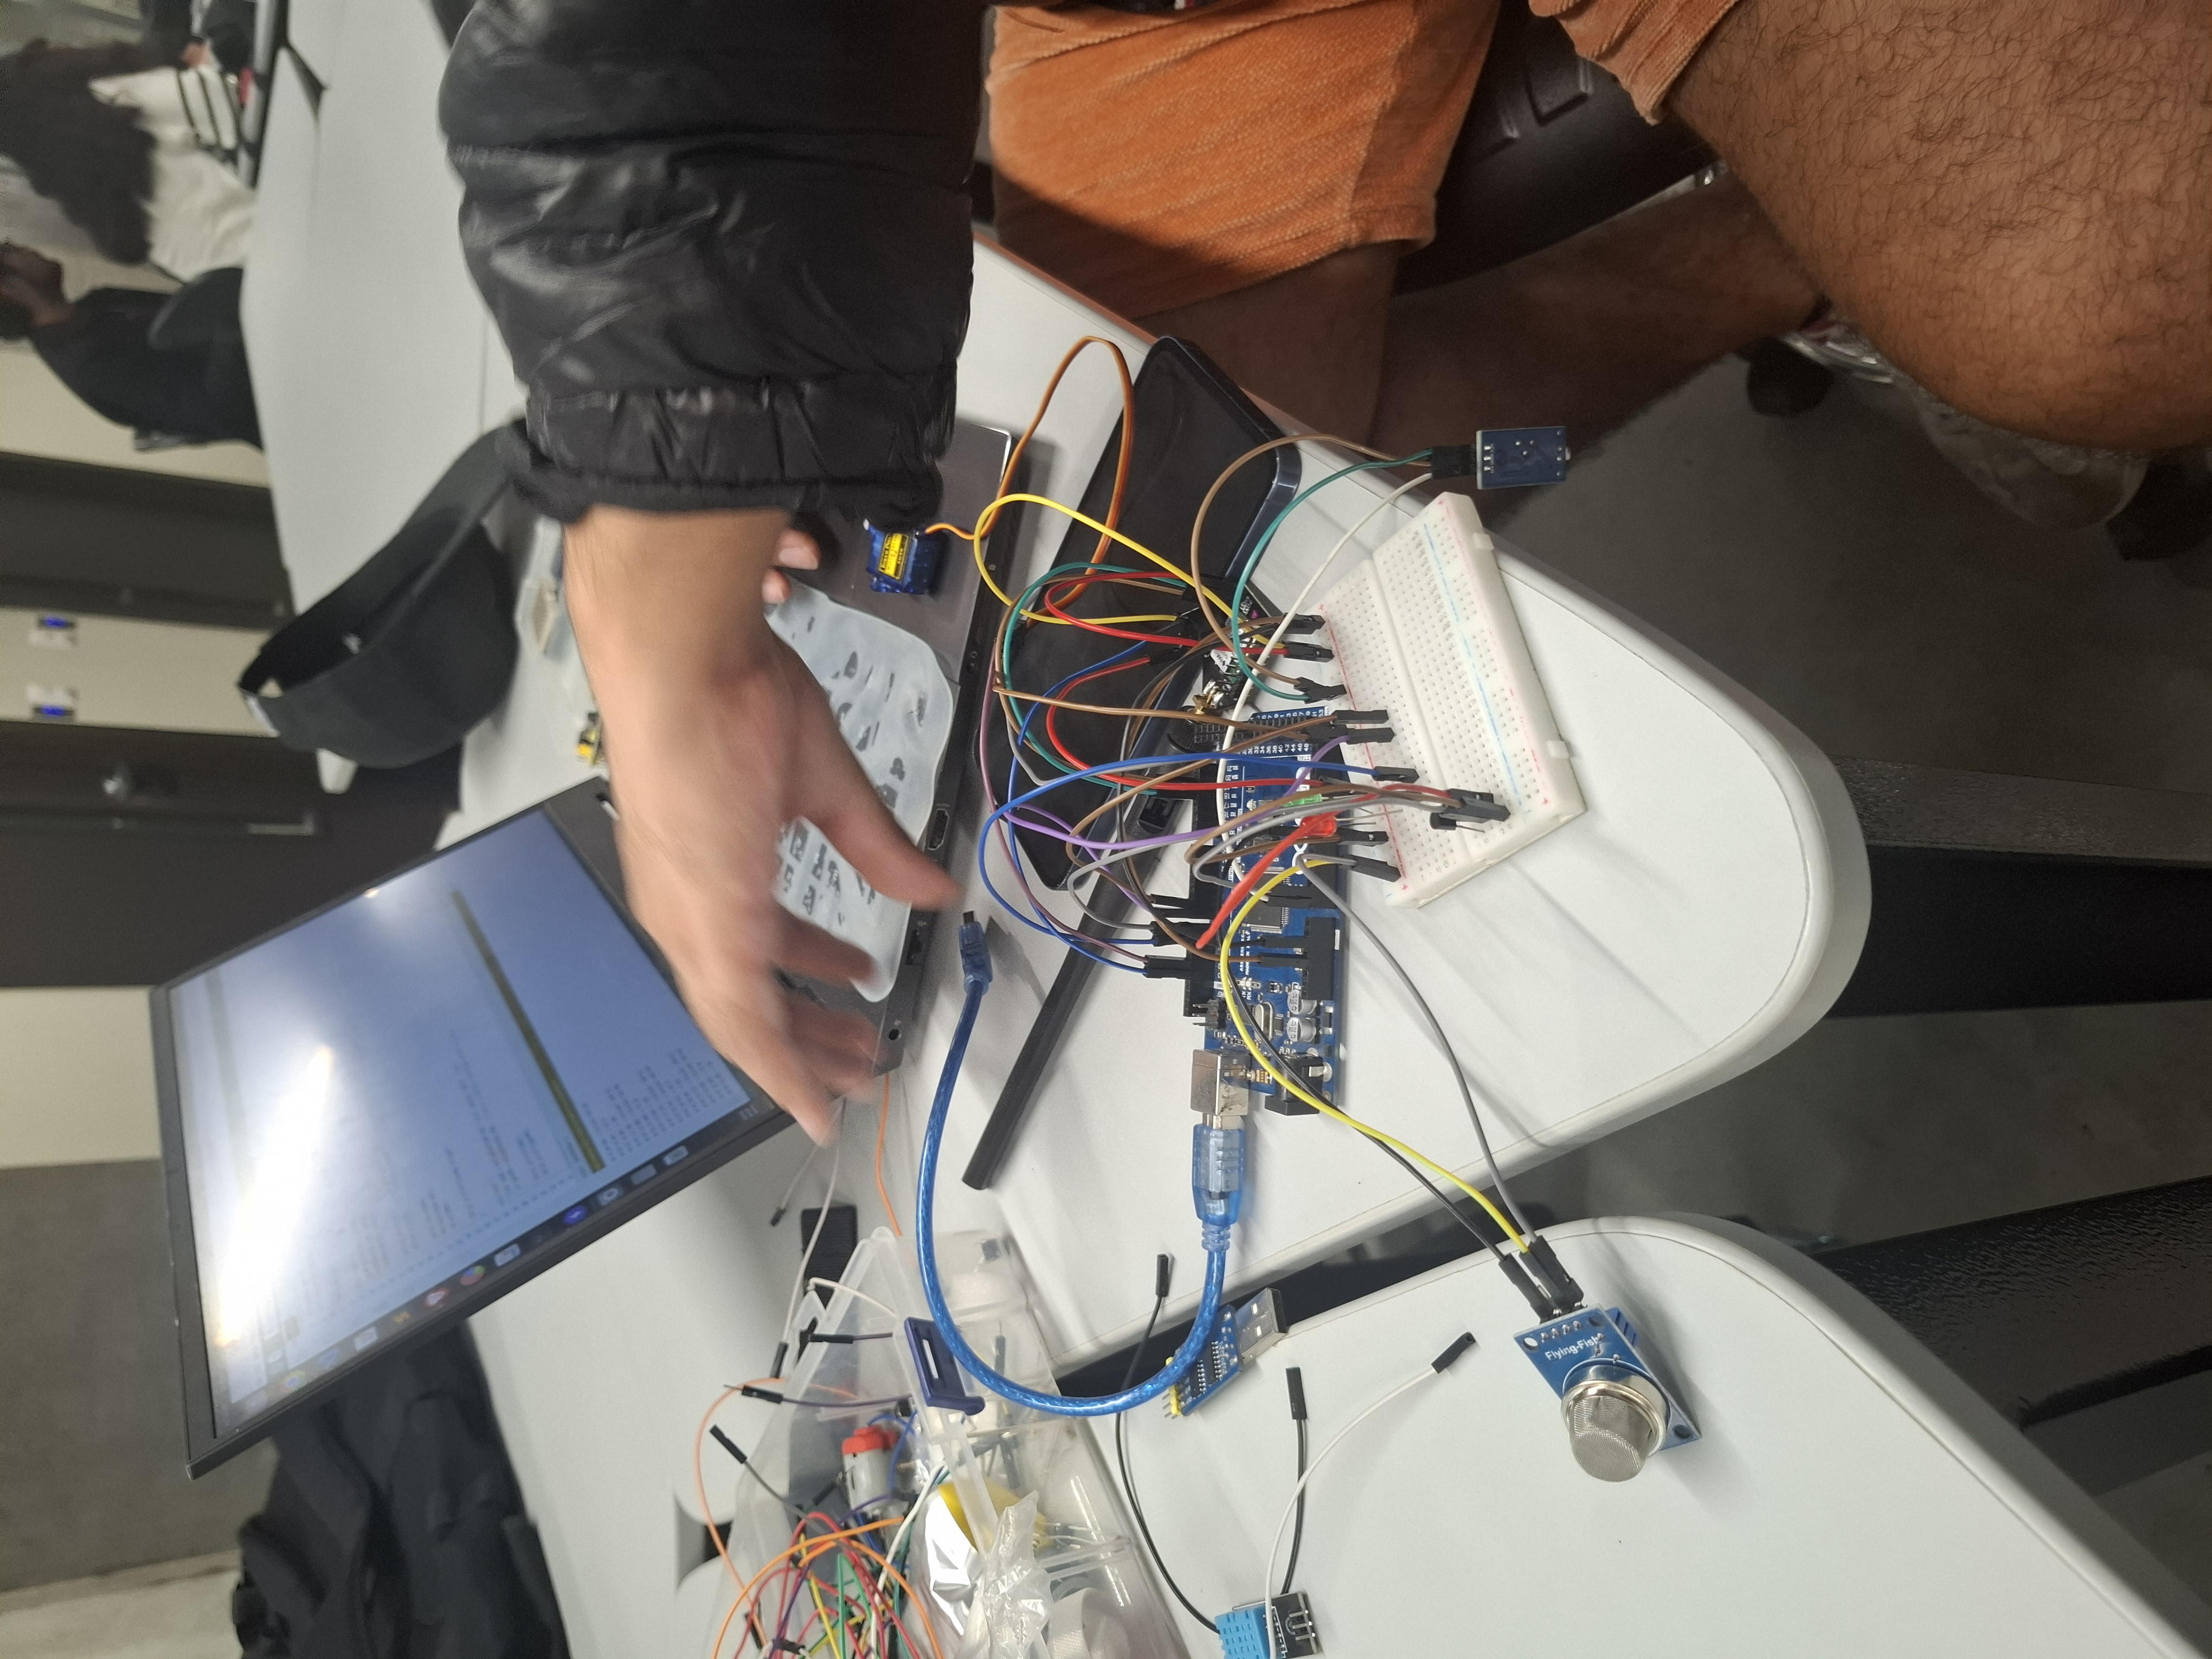
\includegraphics[width=0.85\textwidth]{./img/fuga_gas_impl.jpg}
    \caption{...}
    \label{fig:fuga_gas_impl}
\end{figure}

% TODO: Implementación de ambos sistemas y demostrar el funcionamiento de ambos.
% TODO: Mensajes enviados, en sus respectivas frecuencias.
% TODO: Los sistemas deben estar conectados a laptops diferentes, a fin de demostrar la comunicación inalámbrica.
% TODO: Diagrama de bloques y diagrama de flujo (en clase).
% TODO: Tomar fotos y grabar videos del funcionamiento para su informe.

